\section{Ziel}
Das Ziel dieses Versuchs ist die Bestimmung der Land\'{e}-Faktoren und der Kernspins der Rubidium-Isotope $\ce{^{87}_{}Rb}$ und $\ce{^{85}_{}Rb}$ mit der Hochfrequenzspektroskopie.
Zusätzlich wird das Erdmagnetfeld und das Isotopenverhältnis vermessen und mit theoretischen Werten verglichen.

\section{Theorie}
\label{sec:Theorie}

\subsection{Magnetische Momente und Land\'{e}-Faktoren}
\label{sec:magnetischeMomente}

In der halbklassischen Deutung erzeugt ein Elektron durch seine Kreisbewegung ein Magnetfeld, welches dem magnetischen Moment des Bahndrehimpulses entspricht.
Dieses magnetische Moment koppelt mit dem magnetischen Moment des Spins und es lässt sich folgende Verknüpfung aufstellen
\begin{align}
	\vec{J} = \vec{S} + \vec{L} \;.
	\label{eq:SplusL}
\end{align}
Dabei bezeichnet $\vec{S}$ den Spin, $\vec{L}$ den Bahndrehimpuls und $\vec{J}$ Gesamtdrehimpuls der Elektronenhülle.
Der Gesamtdrehimpuls $\vec{F}$ des Atoms setzt sich aus der Kopplung des Gesamtdrehimpulses $\vec{J}$ und dem Kernspin $\vec{I}$ zusammen:
\begin{align}
	\vec{F} = \vec{J} + \vec{I}
	\label{eq:JplusL}
\end{align}
Die jeweiligen magnetischen Momente stehen antiparallel zu den entsprechenden Vektoren und unterscheiden sich durch einen konstanten Term im Betrag.
\begin{align}
	\vec{\mu}_S&=-g_S\mu_B\vec{S}\\
	\vec{\mu}_L&=-\mu_B\vec{L}\\
	\vec{\mu}_J&=\vec{\mu}_S+\vec{\mu}_L=-g_J\mu_B\vec{J}\\
	\hspace{2cm}
	\vec{\mu}_J&=-g_J\mu_B\vec{S}\\
	\vec{\mu}_I&=-g_I\mu_K\vec{L}
	\label{eq:mu}
\end{align}
Die konstanten Terme vor den Drehimpulsen ergeben sich aus dem Bohrschen Magneton $\mu_B=\frac{e\hbar}{2m_e}$, dem Kernmagneton $\mu_K=\frac{e\hbar}{2m_p}$ und dem Land\'{e}-Faktor $g$, welcher teilchenspezifisch ist.\\

\begin{figure}
\centering
\begin{subfigure}{.5\textwidth}
	\centering
	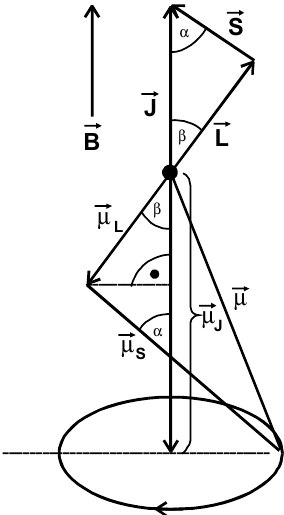
\includegraphics[width=0.45\textwidth]{img/Theorie1.png}
	\caption{}
	\label{fig:Theorie1}
\end{subfigure}%
\begin{subfigure}{.5\textwidth}
	\centering
	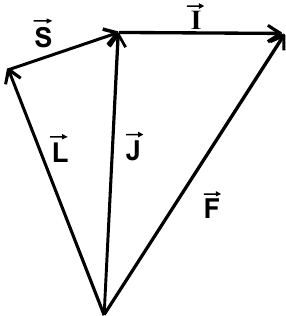
\includegraphics[width=0.45\textwidth]{img/Theorie2.png}
	\caption{}
	\label{fig:Theorie2}
\end{subfigure}
\caption{Geometrische Anordnung der zuvor beschriebenen Drehimpulse und den dazugehörigen magnetischen Momenten.}
\label{fig:geoAnordnung}
\end{figure}

Aufgrund der Präzessionsbewegung um die Gesamtdrehimpulsrichtung $\vec{J}$ mitteln sich alle senkrecht dazu stehenden Komponenten des magnetischen Moments $\vec{\mu}_J$  zeitlich heraus (siehe Abb. \ref{fig:Theorie1}).
Aus den Beträgen der magnetischen Momente
\begin{align}
	|\vec{\mu}_S|&=g_S\mu_B\sqrt{S(S+1)} \\
	|\vec{\mu}_L|&=\mu_B\sqrt{L(L+1)}\\
	|\vec{\mu}_J|&=g_J\mu_B\sqrt{J(J+1)}
	\label{eq:betragmu1}
\end{align}
folgt nach Abbildung \ref{fig:Theorie2} der geometrische Zusammenhang
\begin{align}
	|\vec{\mu}_J| &= |\vec{\mu}_L| \cos{(\beta)}+ |\vec{\mu}_S| \cos{(\alpha)}\;.
	\label{eq:betragJ}
\end{align}
Mit dem magnetische Moment des Kerns
\begin{align}
	|\vec{\mu}_I|&=g_I\mu_k\sqrt{I(I+1)}
\end{align}
und Gleichung \ref{eq:betragJ} lässt sich das magnetische Moments des Atoms unter Berücksichtigung von Abbildung \ref{fig:Theorie2} berechnen:
\begin{align}
	|\vec{\mu}_F|&=|\vec{\mu}_J|\cos{(\vec{J},\vec{F})} + |\vec{\mu}_I|\cos{(\vec{I},\vec{F})}\;.
	\label{eq:betragF}
\end{align}
Der zweite Summand kann aufgrund des Massenunterschieds zwischen Nukleon und Elektron ($\mu_K<<\mu_B$) vernächlässigt werden.
Mit dem Kosinussatz ergibt sich zum Schluss für den Land\'{e}-Faktor des Kerns der Ausdruck:
\begin{align}
	g_F \approx g_J \frac{F(F+1)+J(J+1)-I(I+1)}{2F(F+1)}\;.
	\label{eq:11}
\end{align}


\subsection{Aufspaltung der Energieniveaus}

Die Energieniveaus der Coulomb-Wechselwirkung spalten sich auf unter Berücksichtigung der Spin-Bahn-Kopplung.
Je nach Ausrichtung der magnetischen Momente der Elektronen haben diese eine etwas andere Energie.
Diese Aufspaltung ist deutlich kleiner als die Energiedifferenz zwischen den Anregungsniveaus 1s, 2s usw und wird deshalb als Feinstruktur bezeichnet.
Durch die Kopplung des Kernspins und dem Drehimpuls des Elektronenhülle komm es zu einer weiteren Aufspaltung, die als Hyperfeinstruktur bezeichnet wird.
In einem äußeren Magnetfeld erzeugt das magnetische Moment ein Drehmoment.
Die dabei entstehende potentielle Energie wird als Zeemanenergie $U_\textrm{mag}$ bezeichnet und sorgt für die Aufspaltung der Energieniveaus (Zeeman-Effekt).
In Abbildung \ref{fig:Aufspaltung}) sind die Aufspaltung der verschiedenen Energieniveaus dargestellt.
Da nur die zum Feld parallelen Komponenten von $\vec{\mu}$ relevant sind, kann aufgrund der Richtungsquantelung das magnetische Moment durch die Orientierungsquantenzahl $M$ ersetzt werden, sodass folgt
\begin{align}
	U_\textrm{mag}&=-\vec{\mu} \vec{B}=Mg\mu B\;.
	\label{eq:7}
\end{align}

\begin{figure}
	\centering
	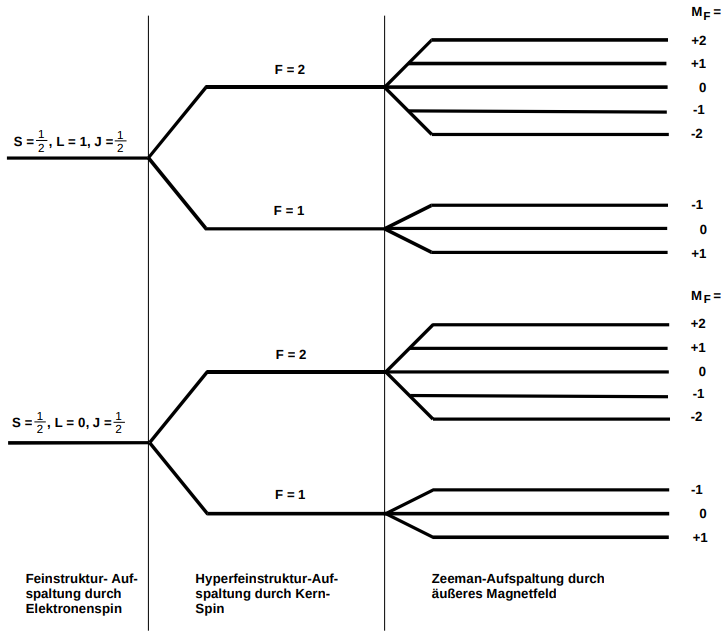
\includegraphics[width=0.55\textwidth]{img/Aufspaltung.png}
	\caption{Aufspaltung der Energieniveaus unterteilt in die Bereiche der Feinstruktur, der Hyperfeinstruktur und der Zeeman-Aufspaltung.}
	\label{fig:Aufspaltung}
\end{figure}

Die Energiedifferenz zwischen den Zeeman-Niveaus unter Berüchsichtichutng der Hyperfeinstruktur beträgt
\begin{align}
	U_\textrm{HF}=M_F g_F\mu_BB.
	\label{eq:8}
\end{align}
Die Näherung der Energiedifferenz in zweiter Ordnung wird als Breit-Rabi-Formel bezeichet
\begin{align}
	U_\textrm{HF}=g_F\mu_BB+g_F^2\mu_B^2B^2\frac{(1-2M_F)}{\Delta E_\textrm{Hy}},
	\label{eq:16}
\end{align}
wobei $\Delta E_\textrm{Hy}$ für die Energiedifferenz der Hyperfeinstruktur zwischen den Niveaus mit den Quantenzahlen $F$ und $F+1$ steht.

\subsection{Optisches Pumpen}
\label{sec:optischesPumpen}

Befinden sich zwei Zustände im thermischen Gleichgewicht, gilt nach der Boltzmann-Verteilung
\begin{equation}
\frac{N_2}{N_1} = \frac{g_2}{g_1} \cdot \exp(-\frac{E_2-E_1}{k_b \cdot T})
\end{equation}
wobei $N_1$, $g_1$ und $E_1$ Dichte, Entartungsgrad und Energie im niederigeren Zustand sind.
$N_2$, $g_2$ und $E_2$ sind die entsprechenden Größen im höheren Zustand.
Eine Besetzungsinversion
\begin{equation*}
	\frac{N_2}{N_1} > \frac{g_2}{g_1}
\end{equation*}
kann also nur vorliegen, wenn sich das System nicht im thermischen Gleichgewicht befindet.
Dafür muss dem System ständig Energie hinzugefügt werden, was in diesem Experiment durch das optische Pumpen erfolgt.
Anhand der von Abbildung \ref{fig:optischesPumpen} soll dieses Prinzip beschrieben werden.

\begin{figure}
	\centering
	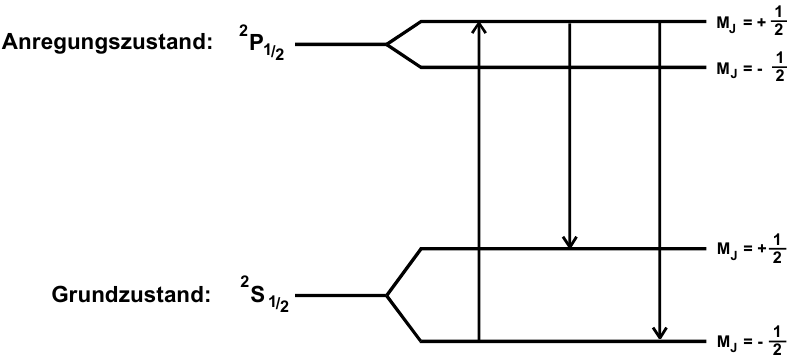
\includegraphics[width=0.55\textwidth]{img/optischesPumpen.png}
	\caption{Aufspaltung der Energieniveaus ohne Hyperfeinstruktur eines Alkali-Atoms mit eingezeichneten erlaubten Übergängen, die durch Anregung bzw. spontane Emission verursacht werden.}
	\label{fig:optischesPumpen}
\end{figure}

Für das erreichen einer Inversion wird rechtszirkular-polarisiertes Licht eingestrahlt.
Aufgrund der Auswahlregel $\Delta M_J=+1$ gehen die Elektronen im niedrigeren Grundzustand $\ce{^{2}_{}S_{1/2}}$ $(M_J=-\frac{1}{2})$ in den angeregten Zustand $\ce{^{2}_{}P_{1/2}}$ $(M_J=+\frac{1}{2})$ über.
Die Elektronen im höheren Grundzustand $\ce{^{2}_{}S_{1/2}}$ $(M_J=+\frac{1}{2})$ werden nicht angeregt, da kein Zustand existiert, der die Auswahlregel erfüllt.
Im angeregten Zustand  $\ce{^{2}_{}P_{1/2}}$ $(M_J=+\frac{1}{2})$ befindliche Elektronen gehen durch spontane Emission, bei der ein Photon emittiert wird, wieder in einen der beiden Grundzustände über.
Dabei ist es annähernd gleich wahrscheinlich, dass der Übergang in den Zustand $\ce{^{2}_{}S_{1/2}}$
$(M_J=-\frac{1}{2})$ und $\ce{^{2}_{}S_{1/2}}$ $(M_J=+\frac{1}{2})$ stattfindet.
Da die Rate der spontanen Emission proportional zu $\omega^3$ ist ($\omega =$ Frequenz des emittierten Photons), erfolgt der Übergang vom Anregungszustand in einen der beiden Grundzustände deutlich schneller als vom höheren Grundzustand in den niedrigeren.
Somit wird der niedrigere Grundzustand $\ce{^{2}_{}S_{1/2}}$ $(M_J=-\frac{1}{2})$ leer gepumpt und es entsteht zu $\ce{^{2}_{}S_{1/2}}$ $(M_J=+\frac{1}{2})$ eine Besetzungszahlinversion.

\subsection{Hochfrequenz-Spektroskopie}
Das im Kapitel \ref{sec:optischesPumpen} angesprochene Verfahren kann unter anderem dazu verwendet werden, die Abstände zwischen zwei Energieniveaus zu vermessen.
Grundsätzlich gibt es zwei Möglichkeiten wie Elektronen, nachdem sich eine Besetzungsinversion eingestellt hat, vom höheren Zustand in den niedrigeren Zustand übergehen können.
Die erste Möglichkeit besteht in der bereits erwähnten spontanen Emission.
Bei der zweiten Möglichkeit, der induzierten Emission, wird ein durch ein Hochfrequenzfeld erzeugtes Photon eingestreut.
Daraufhin wird ein in Polarität, Frequenz und Energie gleiches Photon emittiert und der Zustand geht in der Grundzustand über.
Die dafür benötigte Energie des eingestrahlten Photons entspricht
\begin{align}
	h\nu&=g_J\mu_BB_m\Delta M_J\;.
	\label{eq:hnu}
\end{align}
Welcher der beiden Möglichkeiten dominiert ist frequenzabhängig, in dem vorliegenden Fall kann die spontane Emission vernachlässigt werden.
Um die Breite der Energielücke zu bestimmen wird die Transparenz ausgenutzt, also der Anteil an einfallende Photonen, die nicht absorbiert werden.
Die Tranparenz wird maximal, wenn kein Photon mehr absorbiert wird.
In dem vorliegenden Fall tritt dieses auf, wenn der niedrigere Grundzustand leer gepumpt wird und im hier verwendeten  $\ce{^{87}_{}Rb}$ und $\ce{^{85}_{}Rb}$ keine Photonen mehr zur Anregung absorbiert werden könen.
In Abbildung \ref{fig:TransparenzZeit} ist die entstehende Transparenz gegen die Zeit aufgetragen.
\begin{figure}
	\centering
	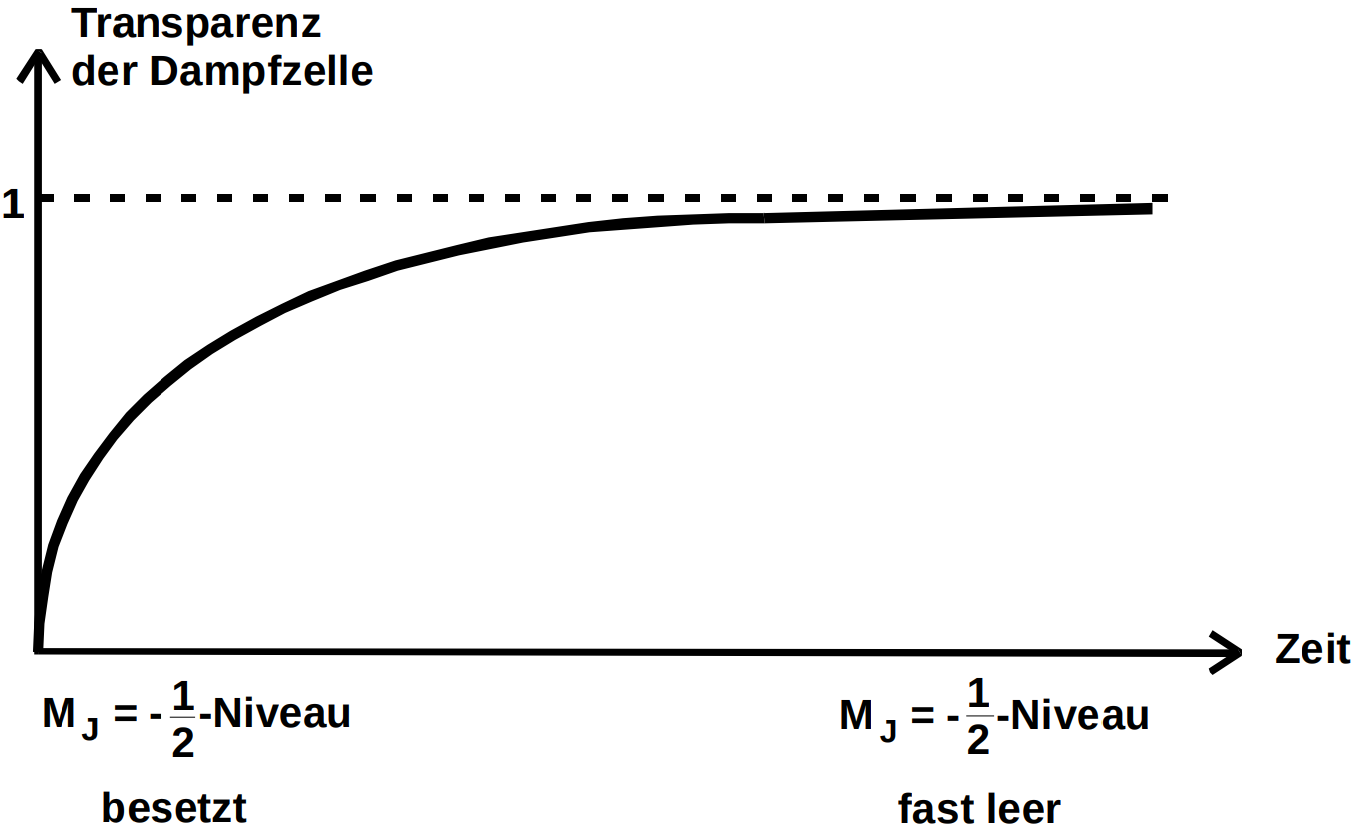
\includegraphics[width=0.475\textwidth]{img/TransparenzZeit.png}
	\caption{Verlauf der Transparenz in einer Alkali-Dampfzelle gegen die Zeit, in der $D_1$-Licht eingestrahlt wird.}
	\label{fig:TransparenzZeit}
\end{figure}
Zur Bestimmung der Breite der Bandlücke wird nun die Resonanzstelle gesucht, die sich in der Transparenz widerspiegelt.
In Abbildung \ref{fig:Resonanz} ist dieses Verhalten bei variierenden Magnetfeld dargestellt.
\begin{figure}
	\centering
	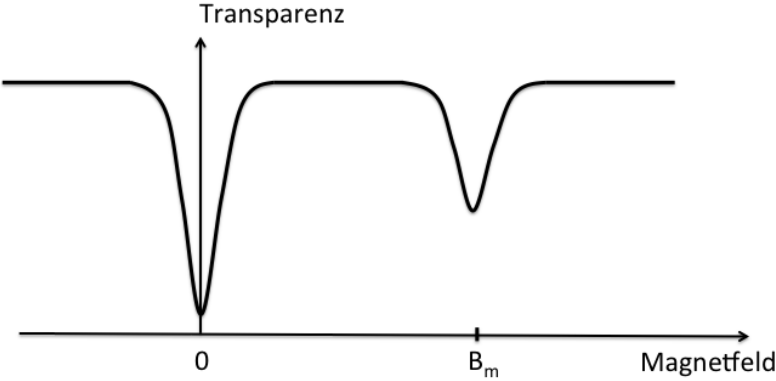
\includegraphics[width=0.475\textwidth]{img/Resonanz.png}
	\caption{Verlauf der Transparenz in einer Alkali-Dampfzelle gegen das Magnetfeld, bei angelegtem Hochfrequenzfeld. \cite{skript}}
	\label{fig:Resonanz}
\end{figure}
Bei verschwindendem Magnetfeld findet keine Zeeman-Aufspaltung statt, wodurch bei $B=0$ die Transparenz auf Null absinkt.
Mit der zweiten Resonanzstelle und Gleichung \ref{eq:hnu} kann somit die Breite der Bandlücke bestimmt werden.
